% -----------------------------------------------------------
%
%  CHAPTER 4  of Quantum information with atoms and photons
%
%  written by Ilaria Delbono + others,Jan 2023
% -----------------------------------------------------------


Electromagnetic waves and, in turn, light come from the coexistence of an electric field $\vec{E}=\vec{E}(\Vec{x},t)$ and a magnetic field $\vec{B}=\vec{B}(\Vec{x},t)$. In vacuum and in absence of sources, they are described by 
the following  Maxwell's Equations: 

\begin{align}
    \vec{\nabla} \cdot \vec{E} &=0, \label{eq:ME1}\\
    \vec{\nabla}\cdot \vec{B} &=0,\label{eq:ME2} \\
    \vec{\nabla}\times\vec{E} &=-\frac{\partial \vec{B}}{\partial t}, \label{eq:ME3}\\
    \vec{\nabla}\times\vec{B} &=\frac{1}{c^2} \frac{\partial \vec{E}}{\partial t}, \label{eq:ME4}
\end{align}
where $c^2 = \varepsilon_0 \mu_0$. 
From these equations, it is possible to find that the electric and magnetic fields satisfy the \textit{Wave Equation}:
\begin{align}
         \left(\nabla^{2}-\frac{\partial^{2}}{\partial t^{2}}\right)\vec{E} &= 0, \\
         \left(\nabla^{2}-\frac{\partial^{2}}{\partial t^{2}}\right)\vec{B} &= 0.
\end{align}
The solutions are
 \begin{equation}
     \vec{E}(\vec{x},t)=\vec{E}_{0} \, e^{i(\vec{k} \cdot \vec{r}-\omega t)} \qquad \text{and} \qquad 
     \vec{B}(\vec{x},t)=\vec{B}_0 \, e^{i(\vec{k} \cdot \vec{r}-\omega t)}. 
 \end{equation}

\section{First Quantization}
\subsection{Electromagnetic potentials and Coulomb gauge}
\label{subsec:3.1.1}
The expressions for $\vec{E}$ and $\vec{B}$ can be derived from a scalar potential $\phi$ and a vector potential $\vec{A}$: 
\begin{equation}
    \vec{E}=-\frac{\partial \vec{A}}{\partial t} - \vec{\nabla}\phi \qquad \text{and} \qquad \vec{B}=\vec{\nabla}\times\vec{A}. 
    \label{eq:empot}
\end{equation}
Maxwell's equations are invariant under the transformations
\begin{align*}
    \phi ~~\longrightarrow ~~ \phi - \frac{\partial f}{\partial t}  \qquad \text{and} \qquad \vec{A}~~\longrightarrow ~~ \vec{A} + \vec{\nabla} f, 
\end{align*}
which are defined for a generic function $f(\vec{r},t)$. This arbitrariness in the definition of $\phi$ and $\vec{A}$ is called \textit{gauge invariance}. In absence of source, it is useful to work with the \textit{Coulomb gauge}: 
\begin{align}
    \phi=0 \qquad \text{and} \qquad \vec{\nabla}\cdot \vec{A}=0. 
\end{align}
This choice allows to deduce the equation of motion for $\vec{A}$. Starting from (\ref{eq:ME4}) and using (\ref{eq:empot}), the left-hand side and the right-hand side become: 
\begin{align}
    \vec{\nabla}\times\vec{B}&=\vec{\nabla}\times(\vec{\nabla}\times\vec{A}) =\vec{\nabla}(\vec{\nabla}\cdot \vec{A})-\nabla^{2}\vec{A} = -\nabla^{2}\vec{A}, \\
    \frac{1}{c^{2}}\frac{\partial \vec{E}}{\partial t} &= -\frac{1}{c^{2}}\frac{\partial }{\partial t} \left( -\frac{\partial \vec{A}}{\partial t} - \vec{\nabla}\phi \right) = \frac{1}{c^2} \frac{\partial^2 \vec{A}}{\partial t^2}. 
\end{align}
From these results, the equation of motion for $\vec{A}$ is
\begin{equation}
    \nabla^{2}\vec{A}-\frac{1}{c^{2}}\frac{\partial^{2}\vec{A}}{\partial t^{2}} \equiv \Box \vec{A} = 0 \label{dal}, 
\end{equation}
which is called \textit{D'Alembert Equation}. The operator $\Box$ is the D'Alembert operator. 

\subsection{Fourier decomposition}
Looking for a solution for (\ref{dal}) is equivalent to solve the Maxwell's Equations for the electric and magnetic fields; therefore, the vector potential is in the form of a monochromatic plane waves. For a better representation of the system, one can consider the Fourier decomposition for $\vec{A}$ in $\omega$-space:
\begin{equation}
\vec{A}(\Vec{r},t)=\frac{1}{2\pi}\int_{-\infty}^{+\infty}{\vec{A}_{\omega}\, e^{-i\omega t}\, d\omega},
\end{equation}
where $\vec{A}_\omega$ is a single-mode solution which frequency $\omega >0$. In order to obtain a real vector potential, it is given by the combination of two waves travelling in opposite directions
\begin{equation}
    \vec{A}_\omega =\alpha(t) \, \Vec{u}(\vec{r})+\text{c.c.} = \alpha_{0} \, e^{-i\omega t} \, \Vec{u}(\vec{r})+ \text{c.c.} 
    \label{eq:Asm}
\end{equation}
and the function $\alpha(t)$ is such that the equation $\ddot{\alpha} + \omega^2 \alpha = 0$ is satisfied. \\
The expression for $\vec{A}_{\omega}$ can be inserted into (\ref{dal}) and the contributions to the left-hand side are: 
\begin{align*}
    \nabla^{2}\Vec{A}_{\omega}&=\alpha_{0}e^{-i\omega t} \, \nabla^{2}\Vec{u}(\Vec{r})+ \text{c.c.} \\
    \frac{\partial^{2}\Vec{A}_{\omega}}{\partial t^{2}}&=(-i\omega)^{2}\alpha_{0}e^{-i\omega t}\, \Vec{u}(\Vec{r})+\text{c.c.}
\end{align*}
and hence
\begin{equation}
    \Box\, {\Vec{A}_{\omega}}=  \left(\nabla^{2}\Vec{u}+\frac{\omega^{2}}{c^{2}}\Vec{u}\right)\alpha_{0}\, e^{-i\omega t}+\text{c.c.} = 0 \qquad \forall t.
\end{equation}
The only way to satisfy this equation is 
\begin{align}
    \left( \nabla^{2} + \frac{\omega^{2}}{c^{2}}\right) \Vec{u} = \left( \nabla^{2} + k^2\right) \Vec{u} = 0,
    \label{eq:Hel}
\end{align}
where in the last step the relation between the wavenumber and the frequency ($k^2 = \omega^2/c^2$) is used. Equation (\ref{eq:Hel}) is called \textit{Helmholtz Equation} and, to solve it, it is necessary to know the boundary conditions. \\
A final note is about the normalization condition for the function $\vec{u}$
\begin{equation}
    \int_{V}{dV \, \abs{\Vec{u}}^{2}}  = 1
    \label{eq:ortho}
\end{equation}
which will be useful in the following. 


\subsection{Classical energy of the electromagnetic field for a single mode}
The energy of the electromagnetic field is given by
\begin{equation}
    \mathcal{E} =\frac{\varepsilon_0}{2} \int_{V} dV \, \left( E^{2}+c^{2}B^{2} \right),
    \label{eq:energy}
\end{equation}
with 
\begin{equation}
    E^2 = \left( \frac{\partial \vec{A}}{\partial t} \right)^2 \qquad \text{and} \qquad B^2 = (\vec{\nabla} \times \vec{A})^2.
    \label{eq:EBsm}
\end{equation}
Notice that $\mathcal{E}$ depends only on $\vec{A}$.

\begin{tcolorbox}
\textbf{Helmholtz theorem} \\
By the Helmholtz theorem, any vector field can be decomposed as $\Vec{E}=\Vec{E}_{\parallel}+\Vec{E}_\perp$ as long as $\abs{\Vec{E}}\rightarrow0$ for $\abs{r}\rightarrow\infty$, where the components are defined in such a way that $\nabla\cdot\Vec{E}_{\perp}=0$ and $\nabla\cross\Vec{E}_{\parallel}=0$. In this case, 
\begin{align*}
    \Vec{E}_{\perp}=-\frac{\partial \vec{A}}{\partial t} \qquad \text{and} \qquad \Vec{E}_{\parallel}=-\nabla\phi
\end{align*}
Therefore, the energy of the electromagnetic field becomes 
\begin{equation*}
    \mathcal{E} = \frac{\varepsilon_0}{2}\int dV \, (E_{\perp}^2+E_{\parallel}^2+c^2B^2).
\end{equation*}
In the Coulomb gauge, the parallel component of the electromagnetic field is neglected and hence
\begin{equation*}
     \mathcal{E} = \frac{\varepsilon_0}{2} \int dV \, (E_{\perp}^2+c^2B^2). 
\end{equation*}
\end{tcolorbox}

Considering the single-mode solution $\Vec{A}_\omega$ which is previously discussed, the terms (\ref{eq:EBsm}) which appear in (\ref{eq:energy}) can be evaluated. In particular, 
\begin{align*}
    \frac{\partial \vec{A}_\omega}{\partial t} &= -i\omega\alpha \Vec{u} +i\omega \alpha^* \Vec{u}^* \\
    \left( \frac{\partial \vec{A}_\omega}{\partial t} \right)^2 &= - \omega^2 \alpha^2 \, \vec{u}\cdot \vec{u} - \omega^2 \alpha^{2} \, \vec{u}^*\cdot \vec{u}^* + 2 \omega^2 \alpha^2 \, \vec{u}\cdot \vec{u}^* 
\end{align*}
and hence
\begin{align*}
    \int_V dV \, E^2 = \int_V dV \left[ - \omega^2 \alpha^2 \, \vec{u}\cdot \vec{u} - \omega^2 \alpha^{2} \, \vec{u}^*\cdot \vec{u}^* + 2 \omega^2 \alpha^2 \, \vec{u}\cdot \vec{u}^* \right]. 
\end{align*}
The term with the magnetic field becomes
\begin{equation*}
    \begin{aligned}
        \int_{V}{dV \, \Vec{B}^{2}} &= \int_{V}dV (\Vec{\nabla}\times\Vec{A})\cdot (\Vec{\nabla}\times\Vec{A}) = \\
        &\underset{\text{(a)}}{=} \int_{V}{dV (\epsilon_{ijk} \, \partial_{j}A_{k})_i B_{i}} = \\ 
        &\underset{\text{(b)}}{=} \bigg[\epsilon_{ijk}\,A_{k}B_{i}\bigg]_{S_j}-\int_{V}{dV \, \epsilon_{ijk}\, A_{k}\partial_{j}B_{i}} = \\
        &\underset{\text{(c)}}{=} \int_{V}{dV\,\Vec{A}\cdot(\Vec{\nabla}\times\Vec{B}}) = \\
        &\underset{\text{(a)}}{=}
        \int_{V}{dV\,\Vec{A} \cdot (\vec{\nabla}\times(\vec{\nabla}\times\Vec{A}))} = \\
        &\underset{\text{(e)}}{=}
        \int_{V}{dV\,\Vec{A} \cdot (-\nabla^{2}\Vec{A})} = \\
        &\underset{\text{(f)}}{=}
        \int_{V}dV \, k^{2}\Vec{A} \cdot \Vec{A} = \\
        &= \int_{V}dV \frac{\omega^2}{c^2} \left[ \alpha^2 \, \vec{u}\cdot \vec{u} + \alpha^{2} \, \vec{u}^*\cdot \vec{u}^* + 2 \alpha^2 \, \vec{u}\cdot \vec{u}^*  \right]
    \end{aligned}
\end{equation*}
where:
\begin{itemize}
    \item[(a)] $\Vec{B}=\Vec{\nabla}\times\Vec{A}$;
    \item [(b)] the integration by part is performed and the first term is negligible because the fields vanish at the boundaries: 
    \begin{align*}
        \bigg[\epsilon_{ijk}\,A_{k}B_{i}\bigg]_{S_j} = 0;
    \end{align*}
    \item[(c)] $\epsilon_{ijk} = - \epsilon_{kji}$ (because it is applied to $\Vec{B}$ and it is antisymmetric);
    \item [(e)] vectorial property $\vec{\nabla}\times(\vec{\nabla}\times\vec{A}) =\vec{\nabla}(\vec{\nabla}\cdot \vec{A})-\nabla^{2}\vec{A} = -\nabla^{2}\vec{A}$; 
    \item[(f)] using the Fourier representation of $\vec{A}$, the Laplace operator returns $k^{2}$. 
\end{itemize}
The expression for $\mathcal{E}$ becomes
\begin{align*}
        \mathcal{E} = 2\varepsilon_{0} \int_{V}{dV \, \Vec{u} \cdot \Vec{u}^{*}\abs{\alpha}^{2}\omega^{2}} = 2\varepsilon_{0} \abs{\alpha}^{2}\omega^{2} \int_{V} dV \, \Vec{u} \cdot \Vec{u}^{*} = 2\varepsilon_{0}\omega^{2}\abs{\alpha}^{2} 
\end{align*}
or, equivalently 
\begin{align}
        \mathcal{E} = 2\varepsilon_{0}\omega^{2}(\alpha_R^2 + \alpha_I^2) = \varepsilon_0 \omega^2 (\alpha^* \alpha + \alpha \alpha^*), 
        \label{eq:en_clas}
\end{align}
where $\alpha_R$ and $\alpha_I$ are the real and imaginary parts of $\alpha$, respectively. 

\subsection{Harmonic oscillator and quantization of energy}

The energy $\mathcal{E}$ of the electromagnetic field in (\ref{eq:en_clas}) can be associated to the classical Hamiltonian for an harmonic oscillator with unitary mass and frequency $\omega$:
\begin{align}
    H = \frac{P^2}{2} + \frac{\omega^2 Q^2}{2}.
\end{align}
The evolution of the system is given by the Hamilton's Equations 
\begin{align}
    \dot{Q} =\frac{\partial H}{\partial P} \qquad \text{and} \qquad \dot{P} =-\frac{\partial H}{\partial Q}
    \label{eq:can}
\end{align}
From this, one may imagine that it is possible to relate $\alpha_R$ and $\alpha_I$ to the canonical variables $P$ and $Q$. This is done by taking 
\begin{align}
    \alpha_R = \frac{Q}{2 \sqrt{\varepsilon_0}} \qquad \text{and} \qquad \alpha_I = \frac{P}{2 \omega \sqrt{\varepsilon_0}}. 
    \label{eq:cooandop}
\end{align}
The operators $\alpha_R$ and $\alpha_I$ must satisfy the Hamilton's Equations (\ref{eq:can}), which become
\begin{align*}
    \dot{Q} = \frac{\partial H}{\partial P} = P \qquad &\implies \qquad  \dot{\alpha}_R = \omega   \alpha_I \\
    \dot{P} = -\frac{\partial H}{\partial Q} = -\omega^2 Q \qquad &\implies \qquad \dot{\alpha}_I = - \omega \alpha_R
\end{align*}
The two relations on the right are trivially verified by noticing that 
\begin{align*}
    \dot{\alpha}(t) = -i\omega \alpha_0 e^{-i\omega t} = \- \omega (\alpha_R + \alpha_I) = -i\omega \alpha_R + \omega \alpha_I, 
\end{align*}
from which
\begin{equation}
    \begin{cases}
        \dot{\alpha}_{R}=\omega\alpha_{I},\\
        \dot{\alpha}_{I}=-\omega\alpha_{R}.
    \end{cases}
\end{equation}

The quantum version of the classical Hamiltonian (\textit{first quantization}) can be obtained simply using the correspondence rule to replace $Q$ and $P$ by their operator equivalents $\hat{Q}$ and $\hat{P}$: 
\begin{align}
    \hat{H} = \frac{\hat{P}^2}{2} + \frac{\omega^2 \hat{Q}^2}{2}. 
    \label{eq:quantumH}
\end{align}
These operators must satisfy the canonical commutation relation $[\hat{Q},\, \hat{P}] =  i \hbar \mathbb{I}$.
The solution is obtained following the usual resolution for the harmonic oscillator problem, which is based on the introduction of ladder operators
\begin{align*}
    \hat{a} = \sqrt{\frac{\omega}{2 \hbar}} \left( \hat{Q} + \frac{i}{\omega} \hat{P} \right) \qquad \text{and} \qquad \hat{a}^\dagger = \sqrt{\frac{\omega}{2 \hbar}} \left( \hat{Q} - \frac{i}{\omega} \hat{P} \right),
\end{align*}
which satisfy the commutation relation $[\hat{a},\hat{a}^\dagger] = \mathbb{I}$. With this procedure, the quantum Hamiltonian (\ref{eq:quantumH}) becomes 
\begin{align}
    \hat{H} = \frac{\hbar \omega}{2} \left( \hat{a}^\dagger \hat{a} + \hat{a} \hat{a}^\dagger \right) =  \hbar \omega \left( \hat{a}^\dagger \hat{a} + \frac{1}{2}\right) = \hbar \omega \left( \hat{N} + \frac{1}{2}\right), 
    \label{eq:hamHO}
\end{align}
where $\hat{N}$ is the number operator which counts the number of photons in the field.
The Hilbert space for this Hamiltonian is the \textit{Fock state}, which is made of vectors defined starting from the Fock vacuum state $\ket{0}$: 
\begin{align}
    \ket{n} = \frac{\left( \hat{a}^\dagger\right)^n}{\sqrt{n!}} \ket{0}. 
\end{align}



%In second quantizazion will be specified the nature of Hamiltonian in Harmonic Oscillator in terms of creation ($a$) and annichilation ($a^{\dagger}$) operator. With this knowledge can be shown that $\alpha=\sqrt{\frac{\hbar}{2\omega\epsilon_{0}}}a$.


\section{Second Quantization}
\newcommand{\A}{\hat{\vec{A}}}
\newcommand{\dsr}[1]{\hat{a}_{#1}}
\newcommand{\crt}[1]{\hat{a}^{\dagger}_{#1}}
\newcommand{\ur}[1]{\vec{u}_{#1}(\vec{r})}
\newcommand{\urc}[1]{\vec{u}_{#1}^{\ast}(\vec{r})}
\newcommand{\ub}[1]{\vec{u}_{#1}}
\newcommand{\ubc}[1]{\vec{u}_{#1}^{\ast}}
\newcommand{\ux}[3]{\vec{u}(#1, #2, #3)}
\newcommand{\N}{\crt{} \dsr{}}
\newcommand{\dr}{\vec{dr}^{3}}
\newcommand{\pw}{e^{i \vec{k} \cdot \vec{r}}}
\newcommand{\pwc}{e^{-i \vec{k} \cdot \vec{r}}}

%Considering a single mode of the solution of D'Alembert equation (with boundaries conditions):
%\begin{equation}
%    \left( \nabla^{2} + \frac{\omega^{2}}{c^{2}} \right)\ur{}=0
%\end{equation}
%we get the following hamiltonian:
%\begin{equation}
%    \hat{H}_{EM} = \hbar \omega \left( \crt{} \dsr{} + \frac{1}{2} \right) \text{      with   } N=\N
%\end{equation}
%We found out in the previous section that we can rewrite $\hat{\vec{A}}$ for a single mode as:
%\begin{equation}
%    \A = \sqrt{\frac{\hbar}{2 \epsilon_{0} \omega}}(\urc{} \crt{} + \ur{} \dsr{})
%\end{equation}
%which we will refer to as the \textbf{Quantum Field vector} (QF).\\
%Let be $\ur{n}$ a full set of solutions for eq. 3.15 such that is a complete basis for $\mathbb{R}^3$. 
%This is possible because the Laplace operator is hermitian and linear. The orthonormalization condition %would be:
%\begin{equation}
%    \int \dr \urc{n}\ur{n'} = \delta_{n, n'}
%\end{equation}
%with:
%\begin{equation*}
%    \left( \nabla^{2} + \frac{\omega^{2}}{c^{2}} \right)\ur{n}=0
%\end{equation*}

A different approach (which leads to the same results) can be followed if one promotes the classical amplitudes $\alpha$ and $\alpha^*$ in the vector potential to operators. Indeed, from the relations in (\ref{eq:cooandop}), the promotion of $Q$ and $P$ to operators can be transferred to $\alpha_R$ and $\alpha_I$ to obtain an expression for $\hat{\alpha}$: 
\begin{align}
    \hat{\alpha} = \hat{\alpha}_R + i \hat{\alpha}_I = \frac{\hat{Q}}{2 \sqrt{\varepsilon_0}} + i \frac{\hat{P}}{2 \omega \sqrt{\varepsilon_0}},
\end{align}
which in terms of ladder operators becomes
\begin{align}
    \hat{\alpha} = \frac{1}{2} \sqrt{\frac{\hbar}{2 \varepsilon_0 \omega}} \left[ \dsr{} + \crt{} - \left( \crt{} - \dsr{} \right) \right] = \sqrt{\frac{\hbar}{2 \omega \varepsilon_0}} \dsr{}. 
    \label{hata}
\end{align}
Substituting (\ref{hata}) in (\ref{eq:en_clas}), the quantum Hamiltonian obtained with this approach is equivalent to the one in (\ref{eq:hamHO}). \\
The vector potential (\ref{eq:Asm}) can be written as 
\begin{equation}
    \A_\omega(\vec{r},t) = \sqrt{\frac{\hbar}{2 \varepsilon_{0} \omega}}\left[ \urc{} \, \crt{}(t) + \ur{} \, \dsr{}(t) \right], \label{eq:potsm}
\end{equation} 
in which is underlined the fact that $\ur{}$ remains a function of $\hat{r}$, while the temporal dependence is contained in $\hat{a}(t)$ and $\hat{a}^\dagger(t)$. From this expression, it is possible to obtain the electric field for a single mode using 
\begin{align*}
    \hat{\vec{E}}_\omega (\vec{r}, t) = - \frac{\partial \vec{A}_\omega}{\partial t}. 
\end{align*}
To obtain final expression, the time-derivative of the creation and destruction operators must be evaluated:
\begin{align*}
    \frac{d \crt{}}{d t} =& \frac{i}{\hbar}\left[\crt{}, \hat{H}\right] = -i \omega\crt{}, \\
    \frac{d \dsr{}}{d t} =& \frac{i}{\hbar}\left[\dsr{}, \hat{H}\right] = i \omega \dsr{},
\end{align*}
where the commutation relation between $\dsr{}$ and $\crt{}$ is used. Therefore, the electric field becomes 
\begin{align}
    \hat{\vec{E}}_\omega(\vec{r}, t) = -i \sqrt{\frac{\hbar \omega_k}{2 \epsilon_0}} \left[\urc{} \, \crt{}(t)  - \ur{} \, \dsr{}(t) \right]. 
    \label{eq:elfield_sm}
\end{align}
These results for $\hat{\vec{A}}$ and $\hat{\vec{E}}$ show that the vector potential and the electric field are now \textit{quantum field vectors}, indeed they are operators defined in each space point. \\

After this discussion, one can conclude that there is an important difference between a quantized field theory and non-relativistic quantum mechanics: in the former, it is the amplitudes (and hence the fields) which are operators and the position and time coordinates are ordinary numbers, whereas in the latter the position coordinates are operators. 

\subsection{Multi-mode Hamiltonian}
The previous part can be extended to the multi-mode case. In order to do this, consider a full set of solutions $\ur{n}$ for equation (\ref{eq:Hel}) and notice that it forms a complete basis in $\mathbb{R}^3$ (this is possible because the Laplace operator is hermitian and linear). The normalization condition becomes
\begin{equation}
    \int \dr \urc{n} \, \ur{n'} = \delta_{n, n'}. 
    \label{eq:norm_cond}
\end{equation}
and the quantum field vectors in (\ref{eq:potsm}) and (\ref{eq:elfield_sm}) are written as 
\begin{align}
    \A &= \sum\limits_{n} \sqrt{\frac{\hbar}{2 \epsilon_{0} \omega_{n}}}\left[ \ubc{n} \crt{n} + \ub{n} \dsr{n} \right] \\
    \hat{\vec{E}} &= - i \sum\limits_{n} \sqrt{\frac{\hbar \omega_n}{2 \epsilon_0}} \left[ \ubc{n} \crt{n} - \ub{n} \dsr{n} \right]
\end{align}
and the Hamiltonian becomes a collection of uncoupled harmonic oscillators
\begin{equation}
    \hat{H} = \sum\limits_{n} \hbar \omega_n \left( \crt{n} \dsr{n} + \frac{1}{2} \right). 
    \label{eq:Hmm}
\end{equation}
The energy levels obtained from this Hamiltonian are shown in figure (\ref{fig:HspaceQF}), while the commutation relation between $\dsr{n}$ and $\crt{n}$ becomes $\left[\dsr{n'},\crt{n}\right] = \mathbb{I} \delta_{n,n'} $. 

\begin{figure}[h!]
\centering
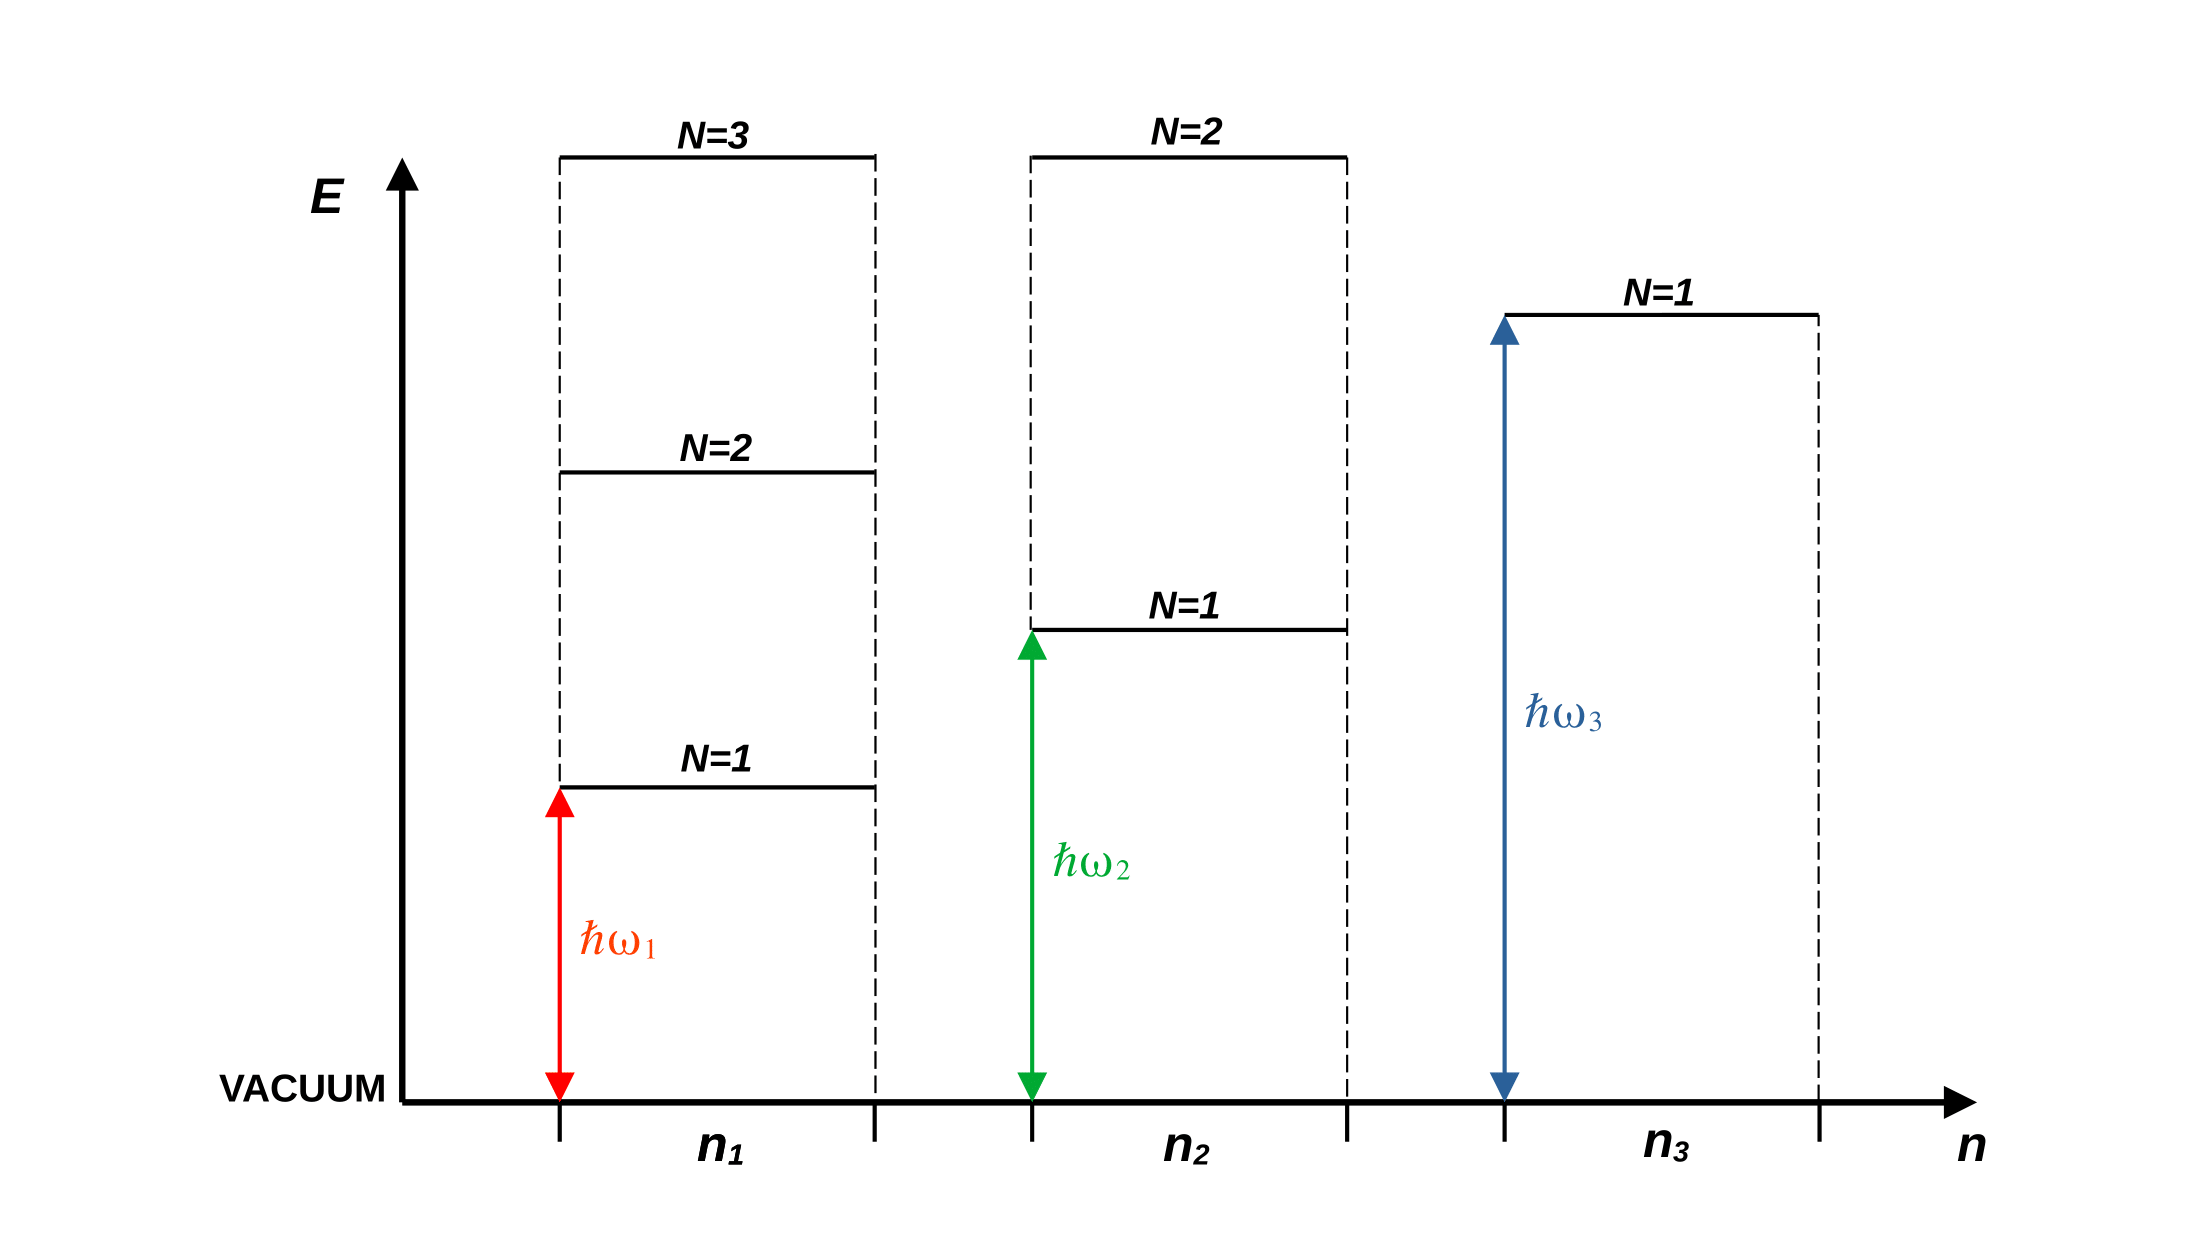
\includegraphics[width=0.8\linewidth]{images/Hilbert_space_QF.png}
\caption{Representation of the energy levels obtained from \ref{eq:Hmm}. Note that, in reality, every mode has a different value of point-zero energy.}
\label{fig:HspaceQF}
\end{figure}

\section{Electromagnetic fields in cavities}

\subsection{Cubic volume with periodic boundary conditions}
Consider a cubic volume $V=L_x L_y L_z$ with periodic boundary conditions, i.e. such that
\begin{align}
    \ux{x}{y}{z} &= \ux{x+L_x}{y}{z}, \\
    \ux{x}{y}{z} &= \ux{x}{y+L_y}{z}, \\
    \ux{x}{y}{z} &= \ux{x}{y}{z+L_z},
\end{align}
and take
\begin{align}
    \ur{}= u(\vec{r}) \vec{\epsilon} =  \frac{1}{\sqrt{V}}  \pw \vec{\epsilon}
\end{align}
as a possible solution for equation (\ref{eq:Hel}), where $\vec{\epsilon}$ is a tridimensional unitary vector. It is straightforward to prove that it is a solution 
\begin{align*}
    \left( \nabla^2  + \frac{\omega^2}{c^2} \right)\vec{\epsilon} \frac{1}{\sqrt{V}}  \pw = 
    \frac{\vec{\epsilon}}{\sqrt{V}} \left[ (i \vec{k})^2 + \frac{\omega^2}{c^2} \right] \pw = 
    \frac{\vec{\epsilon}}{\sqrt{V}} \left[ -k^2 + \frac{\omega^2}{c^2} \right] \pw = 0
\end{align*}
where in the last step the dispersion relation in vacuum ($\omega = k c$) is used.  \\
 
An important condition on $\vec{k}$ is found out from the periodic boundary conditions, indeed considering the one in the $z$-direction
\begin{gather*}
    \ux{x}{y}{z} = \ux{x}{y}{z+L_z} \quad \Longleftrightarrow \quad 
    \frac{\vec{\epsilon}}{\sqrt{V}} e^{i(x k_x + y k_y + z k_z)} = \frac{\vec{\epsilon}}{\sqrt{V}} e^{i(x k_x + y k_y + z k_z + L_z k_z)}
\end{gather*}
from which 
\begin{align}
    1 = e^{i L_z k_z} \quad \implies \quad k_z L_z = 2 \pi n_x \quad \Longleftrightarrow \quad k_z = \frac{2\pi}{L_z} n_z, \quad n_x \in \mathbb{Z}. 
    \label{eq:boundary}
\end{align}
One can repeat the same calculations for each direction. At the end, $\vec{k}$ must be:
\begin{equation}
    \vec{k} = \left( \frac{2 \pi}{L_x} n_x, \frac{2 \pi}{L_y} n_y, \frac{2 \pi}{L_z} n_z\right) \qquad \text{with} \qquad n_x, n_y, n_z \in \mathbb{Z}. 
\end{equation}
The numbers $n_x$, $n_y$ and $n_z$ are not independent, indeed the Coulomb gauge implies that
\begin{align*}
     \vec{\nabla} \cdot \vec{A} = \vec{\nabla} \cdot \ur{} = \vec{\nabla} \cdot \left(  \frac{\vec{\epsilon}}{\sqrt{V}} \pw \right) =
    \frac{\vec{\epsilon}}{\sqrt{V}} \cdot (i \vec{k}) \pw = 0 
\end{align*}
from which 
\begin{equation}
    \vec{\epsilon} \cdot \vec{k} = 0,
\end{equation}
where $\vec{\mathbf{\epsilon}}$ is the \textit{polarisation vector}. This relation shows that the electromagnetic field in vacuum is a transverse field. \\
The vector $\epsilon$ can be decomposed as the sum of two given basis vectors $\vec{\epsilon_{\lambda}}$ with $\lambda = 1, 2$ which lie in the plane perpendicular to $\vec{k}$, as shown in figure \ref{fig:Pol}. 
\begin{figure}[h!]
\centering
    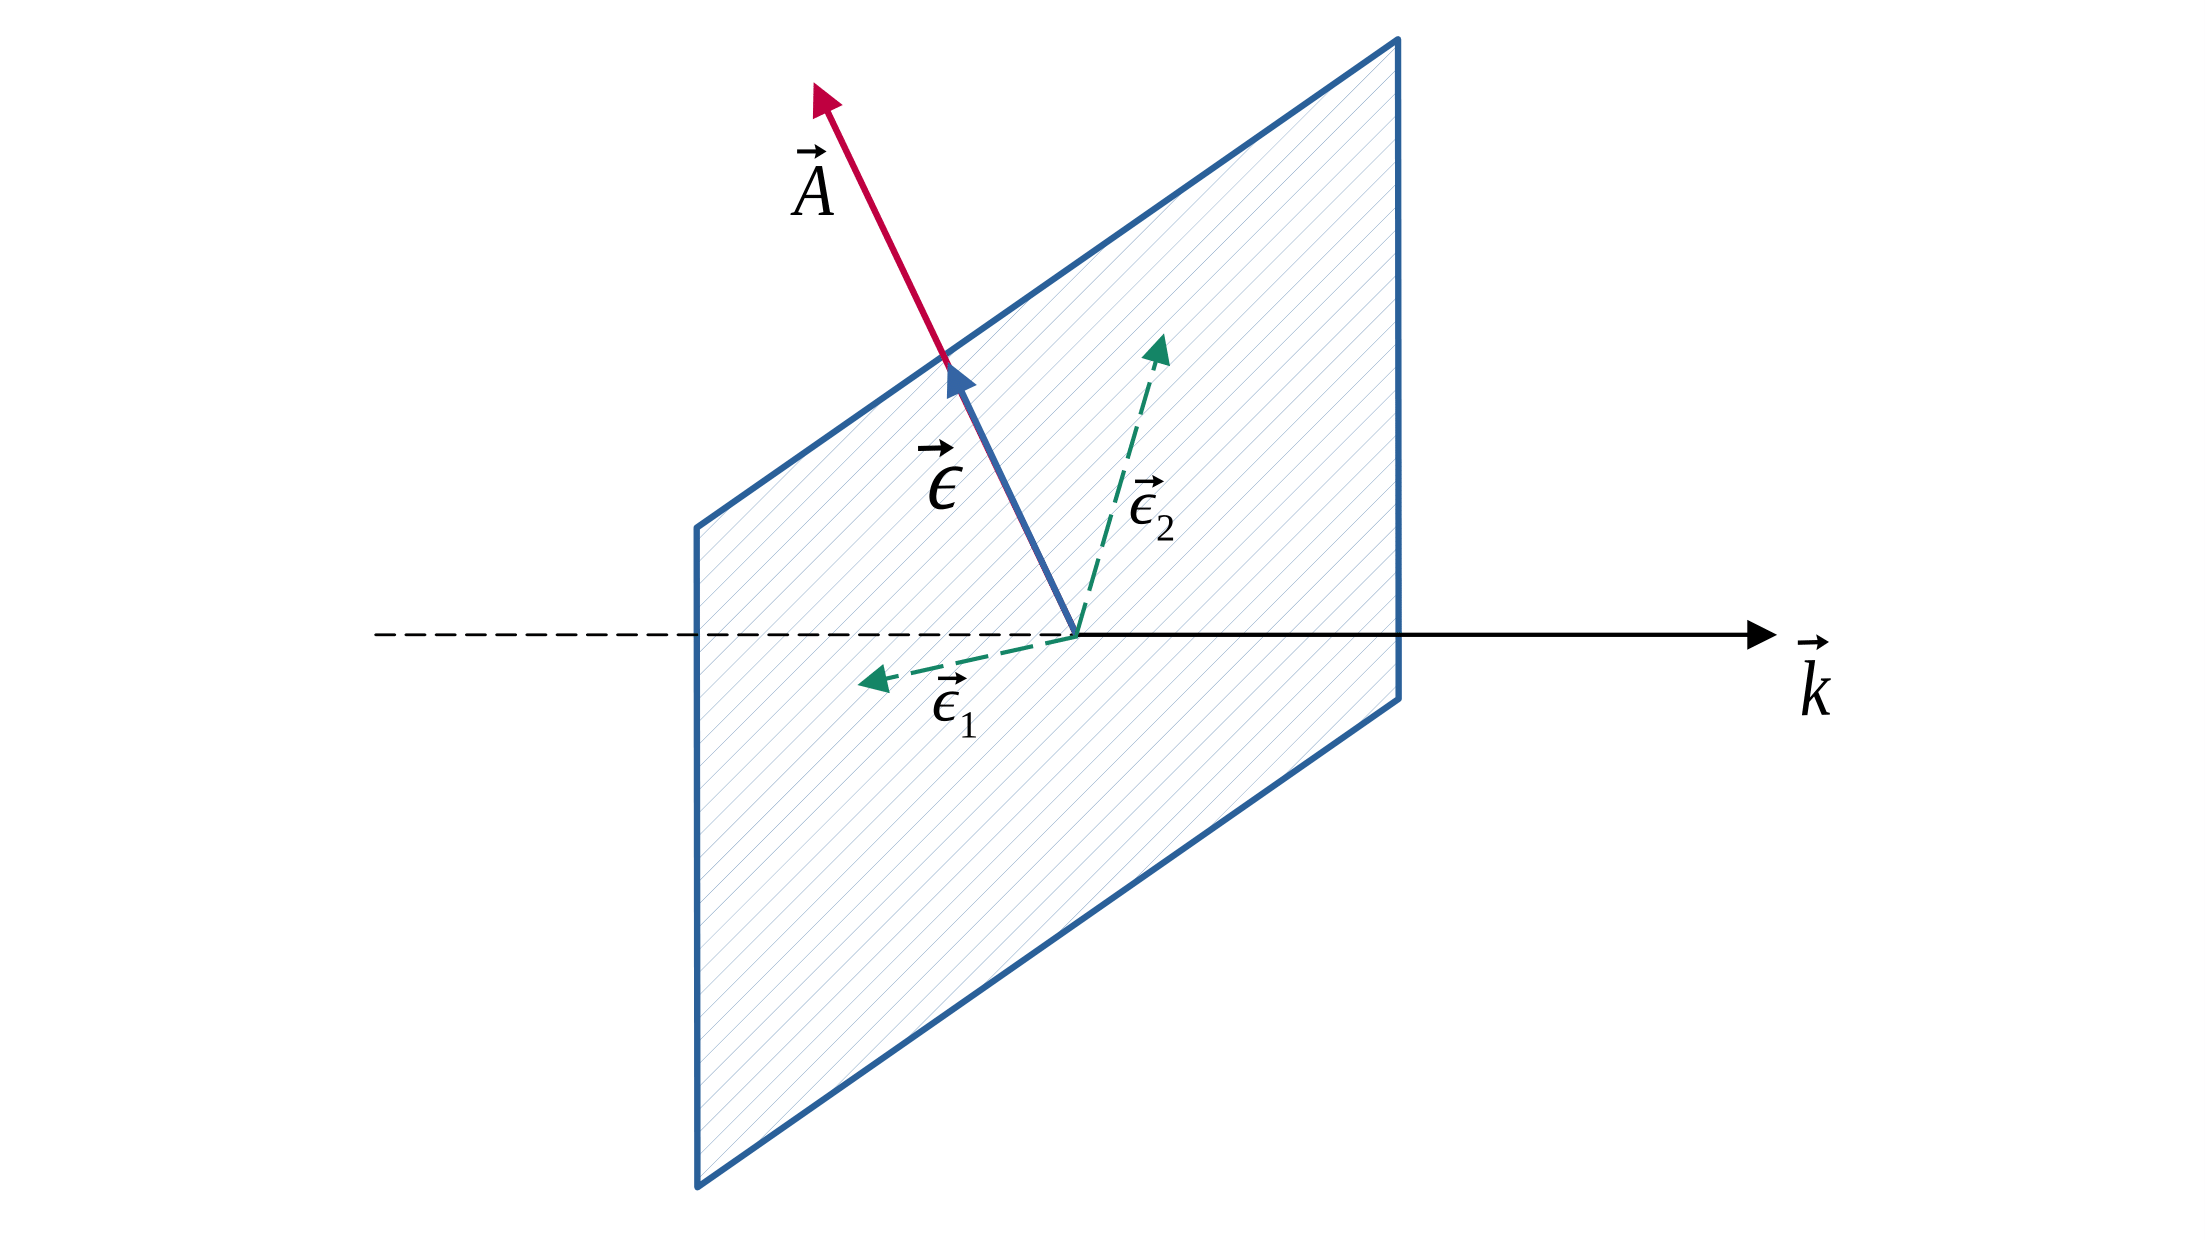
\includegraphics[width=0.78\linewidth]{images/Polarisation.png}
    \caption{Decomposition of the polarization vector $\vec{\epsilon}$ in the plane parallel to the propagation vector $\vec{k}$.}
    \label{fig:Pol}
\end{figure}

Therefore, the quantum field vectors and the Hamiltonian can be defined in terms of $\vec{k}$ and $\lambda$:
\begin{align}
     \A(\vec{r}, t) &= \sum\limits_{\vec{k}, \lambda} \sqrt{\frac{\hbar}{2 \varepsilon_{0} \omega_{k}}} \vec{\epsilon}_\lambda \left[ u_{\vec{k}, \lambda}^* \crt{\vec{k}, \lambda}   + u_{\vec{k}, \lambda} \dsr{\vec{k}, \lambda} \right], \label{eq:potvec}\\
     \hat{\vec{E}}(\vec{r}, t) &= -i \sum\limits_{\vec{k}, \lambda} \sqrt{\frac{\hbar \omega_k}{2 \varepsilon_0}} \vec{\epsilon}_{\lambda} \left[u_{\vec{k}, \lambda}^* \crt{\vec{k}, \lambda}  - u_{\vec{k}, \lambda} \dsr{\vec{k}, \lambda} \right], \label{eq:elfield}\\
     \hat{H} &= \sum\limits_{\vec{k}, \lambda} \hbar \omega_{\vec{k}} \, \crt{\vec{k}, \lambda} \dsr{\vec{k}, \lambda}. \label{eq:Hlight }
\end{align}
Notice that: 
\begin{itemize}
    \item the vacuum energy terms in the Hamiltonian is dropped with respect to the previous expressions (with a  finite number of dimensions that would not be a problem since the presence of a constant does not change the dynamics of the system; 
    \item the commutation relation between $\crt{\vec{k}, \lambda}$ and $\dsr{\vec{k}', \lambda'}$ becomes 
    \begin{equation}
        \left[\dsr{\vec{k}, \lambda}, \, \crt{\vec{k}', \lambda'}\right] = \mathbb{I} \delta_{\vec{k}, \vec{k'}} \delta_{\lambda, \lambda'}.
    \end{equation}
\end{itemize}

Finally, assuming $\vec{k} = (2 \pi/ L)\, \vec{n}$ and $\vec{k} \neq \vec{k'}$, the orthonormalization condition (\ref{eq:ortho}) is expressed as:
\begin{align*}
    \vec{\epsilon_{\lambda}} \cdot \vec{\epsilon_{\lambda'}} \int dV \frac{\pw}{\sqrt{V}} \frac{e^{-i\vec{k}'\cdot\vec{r}}}{\sqrt{V}} =
    &= \vec{\epsilon_{\lambda}} \cdot \vec{\epsilon_{\lambda'}}  \frac{1}{V} \int dV \exp{i(\vec{k}-\vec{k'} \cdot \vec{r})} =\\
    &= \vec{\epsilon_{\lambda}} \cdot \vec{\epsilon_{\lambda'}}  \frac{1}{V} \int dV \exp{i 2 \pi  \frac{(\vec{n} - \vec{n'}) \cdot \vec{r}}{L}  } = \\
    &= \vec{\epsilon_{\lambda}} \cdot \vec{\epsilon_{\lambda'}}  \frac{1}{V} \int dV  = \delta_{\lambda, \lambda'} = \delta_{\lambda, \lambda'} \delta_{k, k'}
\end{align*}
where $\delta_{k, k'}$ is introduced since the condition $\vec{k} \neq \vec{k'}$ is imposed at the beginning. \\

With this boundary conditions, one can evaluate the mean value and the variance of the electrical field. Consider a state with $n$ photons with the same mode identified by specific $\vec{k}$ and $\lambda$ and described by the Fock state
\begin{equation}
    \ket{\psi} = \ket{0} \otimes \ket{0} \otimes ... \otimes \ket{n_{\vec{k}, \lambda}} \otimes...\otimes \ket{0} \otimes \ket{0}
\end{equation}
and evaluate $\bra{\psi} \hat{\vec{E}} \ket{\psi} \equiv \langle \hat{\vec{E}} \rangle_\psi$. Remembering that 
\begin{align*}
    \bra{0} \crt{\vec{k}, \lambda} \ket{0} &= 0 \\
    \bra{0} \dsr{\vec{k}, \lambda} \ket{0} &= 0 
\end{align*}
and that 
\begin{align*}
    \bra{n_{\vec{k}, \lambda}} \crt{k, \lambda} \ket{n_{\vec{k}, \lambda}} &= \bra{n_{\vec{k}, \lambda}} \sqrt{n_{k, \lambda}+1} \ket{n_{\vec{k}, \lambda}+1} = 0, \\
    \bra{n_{\vec{k}, \lambda}} \dsr{k, \lambda} \ket{n_{\vec{k}, \lambda}} &= \bra{n_{\vec{k}, \lambda}} \sqrt{n_{k, \lambda}} \ket{n_{\vec{k}, \lambda}-1} = 0,
\end{align*}
one can conclude that $\langle \hat{\vec{E}} \rangle_\psi = 0$ $\forall \ket{\psi}$ and also on the vacuum, i.e. $\langle \hat{\vec{E}} \rangle_0 = 0$. \\
To evaluate the variance of the electrical field, notice that
\begin{equation*}
    \vec{E} \sim \crt{} + \dsr{} \qquad \text{while} \qquad \vec{E}^2 \sim \crt{}\crt{}, \, \dsr{}\dsr{}, \, \crt{}\dsr{}, \, \dsr{}\crt{}
\end{equation*}
and that the only combination of $\crt{}$ and $\dsr{}$ that given an average value which is different from $0$ (also for the vacuum state) is $\langle \dsr{}\crt{} \rangle_{\psi}$. Therefore, 
\begin{equation*}
    \langle \hat{\vec{E}}^2 \rangle_\psi = \sum\limits_{\vec{k}, \lambda} \frac{\hbar \omega_k}{2 \epsilon_0} \abs{\vec{\epsilon_{\lambda}}}^2 \abs{\ub{\vec{k}, \lambda}}^2 \langle \dsr{}\crt{} \rangle_{\psi} \neq 0 \qquad \implies \qquad \langle \hat{\vec{E}}^2 \rangle_0 \neq 0
\end{equation*}
from which 
\begin{equation}
    \Delta \hat{\vec{E}}_0^2 = \langle \hat{\vec{E}}^2 \rangle_0 -\langle \hat{\vec{E}} \rangle_0^2 = \langle \hat{\vec{E}}^2 \rangle_0 \neq 0. 
\end{equation}
This result is in contrast with the one obtained from classical considerations. 

\subsection{Fabry-Perot Cavity}

Consider a volume with dimensions such that $L_z \ll L_x, L_y $ which is delimited by two metallic mirrors located along the $z$-axis and placed perpendicular to it (figure \ref{fig:fp}).
The potential vector is taken with the following spatial dependence:
$${A(\vec{r})} = f_z (z) f_x (x) f_y (y),$$
where $f_x (x)$ and $f_y (y)$ are constant ($n_x =n_y = 0$). This means that the spatial dependence of the vector potential is only on $z$. \\
Since there are mirrors, the periodic boundary condition becomes
\begin{equation}
   \vec{u}(0) = \vec{u}(L_z) = 0, 
\end{equation}
if one is considering a cavity with the first mirror in $z = 0$ and the other in $z = L_z$. An expression for $\vec{u}(\vec{r})$ which satisfies it is 
\begin{equation}
    \ur{}= \vec{u}(z) = \vec{\epsilon}\sqrt{\frac{2}{V}} \sin(k_z z),
\end{equation}
(shown in figure \ref{fig:fp}) and hence the expression for the electric field is obtained from (\ref{eq:elfield}):
\begin{equation}
    \hat{\vec{E}}(\vec{r}, t) = -i \vec{\epsilon}_{\lambda} \sum\limits_{\vec{k}, \lambda} \sqrt{\frac{\hbar \omega_k}{ \varepsilon_0 V}}  \sin(k_z z) \left[ \crt{\vec{k}, \lambda}  - \dsr{\vec{k}, \lambda} \right]. 
    \label{eq:efFP}
\end{equation}

\begin{figure}[H]
\centering
    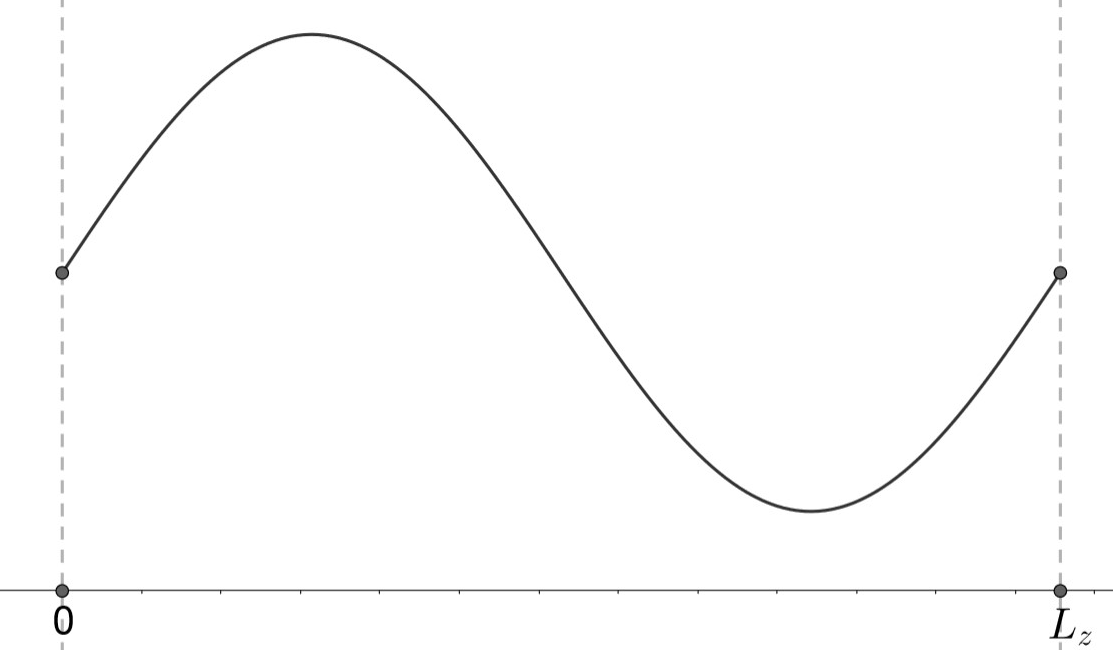
\includegraphics[width=0.65\linewidth]{images/Fabry_Perot.png}
    \caption{Function $\vec{u}(\vec{r})$ for a Fabry-Perot cavity with mirrors in $z = 0$ and $z = L_z$.}
    \label{fig:fp}
\end{figure}

Following the same steps of the previous section:
\begin{itemize}
    \item the boundary conditions (\ref{eq:boundary}) returns: 
    \begin{equation*}
        k_z L_z = \pi n \qquad \implies \qquad k_z =\frac{\pi}{L_z}n \quad \text{and} \quad \vec{u}(z) = \vec{\epsilon} \, \sqrt{\frac{2}{V}} \sin{\left( \frac{\pi}{L_z} n z \right)}
    \end{equation*}
    \item the normalisation condition (\ref{eq:norm_cond}) is verified:
    \begin{equation*}
        \int dV \, \urc{} \, \ur{} = L_x L_y \int dz \, f^{*}(z) f(z) = L_x L_y \int dz \, \frac{2}{V} \sin^2{\left(\frac{\pi}{L_z} n z \right)} = 1.
    \end{equation*}
\end{itemize}
In addition, one can compute the wave dispersion and the distance between two consecutive modes in the cavity:
\begin{equation*}
    \omega_n = c k_z^{(n)} = c \frac{\pi}{L_z}n \qquad \implies \qquad \Delta \omega_n = \frac{c \pi}{L_z}(n+1) - \frac{c \pi}{L_z}n = \frac{c \pi}{L_z}
\end{equation*}

\begin{tcolorbox} [breakable, enhanced]
Taking $L_z = 1$ cm, the separation of modes is about $\Delta \omega_n \simeq  100 $ GHz (microwave-infrared range). \\
The possibility of having a large separation between modes allows to do \textit{single-mode cavity physics}:
\begin{equation*}
    H = \sum\limits_n \hbar \omega_n \crt{n}\dsr{n} \qquad  \longrightarrow \qquad  \hbar\omega \crt{} \dsr{}. 
\end{equation*}
This is useful when an atom inside the cavity emits a single photon at frequency $\omega$, which can be obtained with a proper realisation of the cavity (the modes are \textit{off-resonant} with respect to an atomic transition). 
\end{tcolorbox}

As in the previous subsection, the average value and the variance (evaluated on the vacuum state) of the electric field can be computed. In particular, 
\begin{align*}
    \langle \hat{\vec{E}} \rangle_0 &= 0 \\ 
   \langle \hat{\vec{E}}^2 \rangle_0 &= \frac{\hbar \omega}{2 \epsilon_0} \frac{2}{V} \sin^2\left(\frac{\pi}{L}n z\right) \sim \frac{1}{V}
\end{align*}
and in the centre of the cavity (for $z = L/2$)
$$\langle \hat{\vec{E}}^2 \rangle_0 = \frac{\hbar \omega}{2 \epsilon_0} \frac{1}{V} \neq 0.$$

\section{Coherent states}

It is possible to obtain the states on which the average value of the electric field operator is not null: they are called \textit{coherent states}, usually indicated with $\ket{\alpha_c}$. Using the results of the previous sections, one deduces that they have to satisfy the relations: 
\begin{equation}
    \begin{cases}
        \dsr{} \ket{\alpha_c} = \alpha_c(t) \ket{\alpha_c}, \\
        \bra{\alpha_c} \crt{} = \alpha_c^*(t) \bra{\alpha_c}.
    \end{cases}
\end{equation}
Then, working in the single mode approximation to simplify the steps, one can derive the expression for the average value of the electric field in a Fabry-Perot cavity starting form the expression for $\hat{\vec{E}}$ 
\begin{align}
 \hat{\Vec{E}}(z,t) = - i \ \Vec{\epsilon} \sqrt{\frac{\hbar \omega}{V \varepsilon_0}} \sin\left(k_z z\right) \left[\crt{}(t) - \dsr{}(t)\right]
\end{align}
and evaluating 
\begin{align*}
    \bra{ \alpha_c} \hat{\Vec{E}} \ket{\alpha_c} & =  - i \Vec{\epsilon} \sqrt{\frac{\hbar \omega}{V \varepsilon_0}} \sin(k_z z) \left(\bra{\alpha_c} \crt{} \ket{\alpha_c} - \bra{\alpha_c} \dsr{} \ket{ \alpha_c} \right) \\
    & = - i \Vec{\epsilon} \sqrt{\frac{\hbar \omega}{V \varepsilon_0}} \sin(k_z z) \left(\alpha_c^*(t) - \alpha_c(t)\right) \\
    & = -i  \Vec{\epsilon} \sqrt{\frac{\hbar \omega}{V \varepsilon_0}} \sin(k_z z) \alpha_c(0) \left(e^{\text{i} \omega t} - e^{- \text{i} \omega t}\right) \\
    & = 2 \Vec{\epsilon} \ \sqrt{\frac{\hbar \omega}{V \varepsilon_0}} \sin(k_z z) \sin(\omega t) \alpha_0. 
\end{align*}
In addition to this, one can evaluate the variance of this electric field operator over the coherent states, which leads to:
\begin{align}
    \Delta \hat{\vec{E}}_0^2 & = \left< \alpha_c \right| \hat{\Vec{E}} \cdot \hat{\Vec{E}}\left| \alpha_c \right> - \left( \left< \alpha_c \right| \Vec{E} \left| \alpha_c \right> \right)^2 = \frac{\hbar \omega}{V \varepsilon_0} \sin^2(k_z z), 
\end{align}
since one can prove that
\begin{align*}
    \left< \alpha_c \right| \hat{\Vec{E}} \cdot \hat{\Vec{E}}\left| \alpha_c \right> = \left( \left< \alpha_c \right| \Vec{E} \left| \alpha_c \right> \right)^2 + \frac{\hbar \omega}{V \varepsilon_0} \sin^2(k_z z). 
\end{align*}
In order to evaluate the impact of these fluctuations, one can consider:
\begin{equation}
    \frac{\Delta \hat{\vec{E}}_0^2}{\left| \left< \alpha_c \right| \Vec{E} \left| \alpha_c \right>\right|^2} = \frac{1}{\alpha_c^* (t) - \alpha_c(t)} \sim \frac{1}{\left| \alpha_c(t) \right|} \sim \frac{1}{\left| \alpha_c(0) \right|} 
\end{equation}
This quantity goes to 0 when $\alpha_c(0) \gg 1$, i.e. in a classical situation, in which there is a large number of photons in a coherent state and the addition or the removal of one of them does not have any impact. Indeed $\left| \alpha_c(t) \right|$ corresponds to the expectation value of the number operator $\hat{N}$: 
\begin{equation}
    \left< \alpha_c \right| \hat{N} \left| \alpha_c \right> = \left< \alpha_c \right| \crt{} \, \dsr{} \left| \alpha_c \right> = \left< \alpha_c \right| \alpha^*_c(t) \, \alpha_c(t) \left| \alpha_c \right> = \left| \alpha_c(t) \right|^2.
\end{equation}

\subsection{Glauber's coherent states and occupation probabilities}

\begin{figure}[t!]
\centering
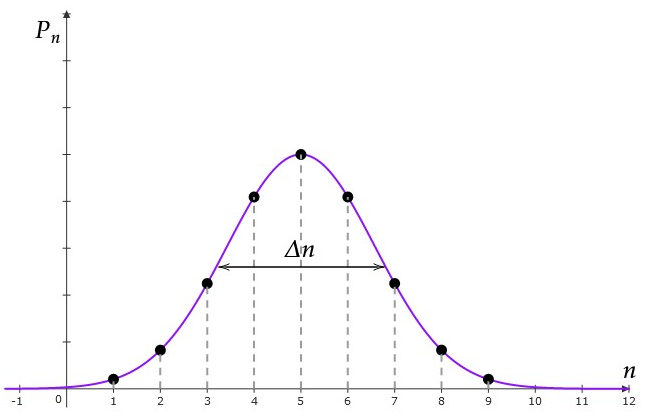
\includegraphics[width=0.7\linewidth]{images/Poisson.png}
\caption{Probability of finding or measuring $n$ photons in a generic coherent state $\ket{\alpha_c}$; for large values of $| \alpha_c|$ it resembles the normal distribution.}
\label{fig:Poisson}
\end{figure}

A generic coherent state $\ket{\alpha_c}$ can be expanded in terms of Fock states
\begin{equation}
    \left| \alpha_c \right> \equiv e^{-\left| \alpha_c \right|^2 / 2} \sum_{n=0}^{\infty} \frac{\alpha_c^n}{\sqrt{n!}} \left| n \right>
    \label{eq:cohstate}
\end{equation}
and it is called \textit{Glauber's coherent state}. \\
From this expression, it is possible to evaluate the probability of finding or measuring $n$ photons in a generic coherent state $\ket{\alpha_c}$: 
\begin{equation*}
    P_n \equiv \left| \bra{n}\ket{\alpha_c}\right|^2 = \left| e^{-\left| \alpha_c \right|^2/2} \frac{\alpha_c^n}{\sqrt{n!}}  \right|^2 =  e^{-\left| \alpha_c \right|^2} \, \frac{\alpha_c^{2n}}{n!},
\end{equation*}
which is a Poisson's distribution with variance $\Delta n = | \alpha_c|$, as shown in figure \ref{fig:Poisson}. 

\subsection{Generation of a coherent state}
A coherent state can be generated starting from the Hamiltonian
\begin{equation*}
    \hat{H} = F \cos (\omega t) \left(\hat{a}^{\dagger} + \hat{a}\right), 
\end{equation*}
where $F$ is the driving force, starting from the vacuum state $\ket{0}$.
